\graphicspath{{fig/model_development/}}

\chapter{Model Development}
\label{cha:model_dev}

In this chapter we shall introduce one of the most popular and well studied agent-based
models in the literature: the Vicsek model. The Vicsek model represents a simple alignment
model in which agents interact with neighbours within some given distance. Despite its
simplicity, this model can produce sophisticated dynamics and exhibits a phase
transition from order to disorder as the amount of noise in the system is regulated.

The Vicsek model, like many other ABMs, implements a discontinuous interaction rule. With
this, the onset of interaction between individuals is very sensitive to small
perturbations in distances. We consider continuous interaction rules as a
biologically-realistic alternative. Such rules ensure the model is more robust to small
perturbations in distances, but without the penalty of extra model complexity.

\section{The Vicsek Model}

The Vicsek model describes the movements of $N$ individuals moving with constant speed
$v$. All movement takes place in a square cell with periodic boundary conditions and side
length $L$. To initialise a simulation all agents are allocated a random position within
the cell, and a random direction of motion. From time $t$ to time $t+1$ agent $i$ updates
its position as:
\begin{equation*}
    \bm{x}_{i, t+1} = \bm{x}_{i, t} + \bm{v}_{i, t},
\end{equation*}
where the velocity $\bm{v}_{i,t}$ is constructed to have speed $v$ and direction of
motion $\theta_{i, t+1}$. The computation of $\theta_{i, t+1}$ describes how agents update
their direction in light of their neighbours' movements, and an additional noise term. In
the Vicsek model the noise is realised from a $\mathcal{U}(-\eta/2, \eta/2)$
distribution. The directional update of agent $i$ can then be expressed as:
\begin{equation}
    \label{eq:vicsek_update}
    \theta_{i, t+1} \given \angmean{\theta}_{i, t}, \eta \sim
                     \mathcal{U}(\angmean{\theta}_{i, t} - \eta/2,
                                 \angmean{\theta}_{i, t} + \eta/2),
\end{equation}
where $\angmean{\theta}_{i, t}$ represents the average direction of motion of agent $i$'s
neighbours at time $t$. As $\angmean{\theta}_{i, t}$ describes a mean of circular
quantities (directions of motion), its computation necessitates the use of the
circular mean:
\begin{equation*}
    \angmean{\theta}_{i, t+1} = \atantwo\bigg(
        \sum_{j=1}^N \omega_{ij, t} \sin\theta_{j,t},
        \sum_{j=1}^N \omega_{ij, t} \cos\theta_{j,t}
    \bigg).
\end{equation*}
With this, $\omega_{ij, t}$ determines the strength of the interaction between agent $i$
and neighbour $j$ at time $t$. In the Vicsek model agents interact with neighbours within
some interaction radius $r$, and so we have:
\begin{equation*}
    \omega_{ij,t} =
    \begin{cases}
        1 & \text{ if } d_{ij, t} \leq r,\\
        0 & \text{ otherwise.}
    \end{cases}
\end{equation*}

\begin{figure}[tb]
    \begin{subfigure}[b]{0.5\textwidth}
        \centering
        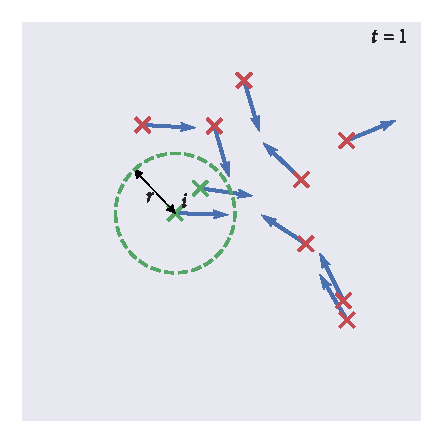
\includegraphics{vicsek_simulation_1.pdf}
    \end{subfigure}%
    \begin{subfigure}[b]{0.5\textwidth}
        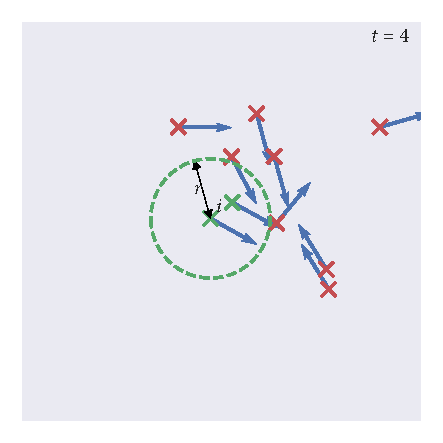
\includegraphics{vicsek_simulation_4.pdf}
    \end{subfigure}
    \begin{subfigure}[b]{0.5\textwidth}
        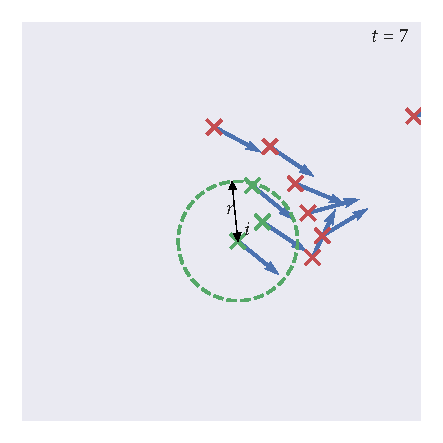
\includegraphics{vicsek_simulation_7.pdf}
    \end{subfigure}%
    \begin{subfigure}[b]{0.5\textwidth}
        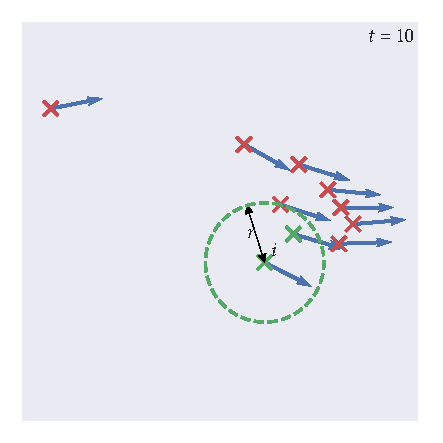
\includegraphics{vicsek_simulation_10.pdf}
    \end{subfigure}
    \caption{Visualisations from a simulation of the Vicsek model. At time $t=1$, $N=10$
        agents are assigned random positions within a square-cell of side length $L=1$.
        Initially, the directions of motion of individuals are realised from a
        $\mathcal{U}(-\pi, \pi)$ distribution. Between time steps agents move with speed
        $v=0.03$, and update directions according to \cref{eq:vicsek_update}, with
        $\eta=\pi/16$. The interaction radius $r$ of agent $i$ is illustrated throughout
        the model simulation. The positions of neighbours within agent $i$'s interaction
        radius are visualised with a green cross. Individuals which lie outside of agent
        $i$'s interaction radius have their positions denoted by a red cross.}
\end{figure}

